% #############################################################################
% This is Chapter 2 - Research Methodology
% !TEX root = ../main.tex
% #############################################################################
\fancychapter{Research Methodology}
\label{chap:methodology}

This chapter presents the research methodologies used in this dissertation, detailing the steps taken in each. The two
methodologies are Systematic Literature Review (SLR) and Design Science Research Methodology (DSRM).

\section{Systematic Literature Review (SLR)} 

The systematic literature review (SLR) conducted in this study follows the guidelines proposed by Kitchenham, who describes a systematic review as “a means of evaluating and interpreting all available research relevant to a particular research question, topic area, or phenomenon of interest.” According to Kitchenham, “systematic reviews aim to present a fair evaluation of a research topic by using a trustworthy, rigorous, and auditable methodology.” These principles ensure that the review process adopted in this work is methodical, transparent, and replicable. The Kitchenham guidelines present three phases:

\begin{itemize}
    \item \textbf{Planning the Review:} Define the motivation, research questions, selection criteria, and review protocol.
    \item \textbf{Conducting the Review:} Apply the protocol to identify and select relevant studies.
    \item \textbf{Reporting the Review:} Synthesize and communicate the findings from the selected literature.
\end{itemize}


\begin{figure}[H]
    \centering
    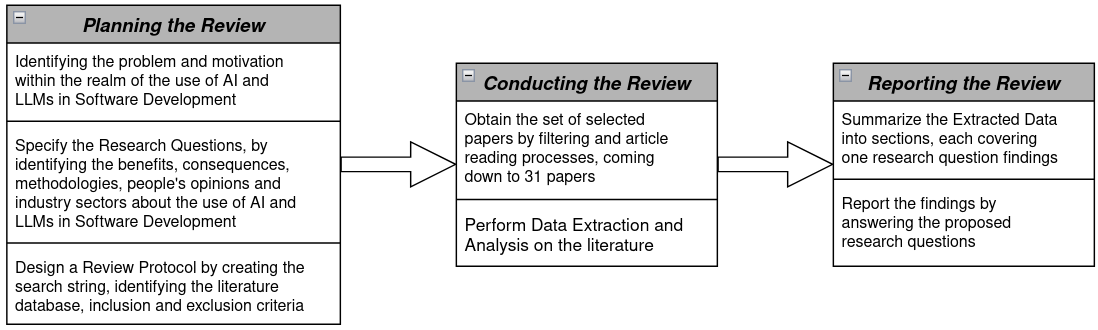
\includegraphics[width=0.85\linewidth]{./Images/phases.png}
    \caption{Three phases of the Systematic Literature Review}
    \label{fig:slr_phases}
\end{figure}

\Cref{fig:slr_phases} illustrates the three phases of the systematic literature review and the activities performed in each phase. The filtering process was conducted through multiple iterations: an initial screening of articles retrieved from the selected database, followed by an abstract-reading iteration to assess relevance, a filtering based on referenced works and Kitchenham’s criteria using introductions and conclusions, and a final full-text review to determine the final set of studies. The SLR methodology was selected as it enables a structured and unbiased collection of existing research on AI-supported software development and its associated frameworks and management practices.s

\section{Design Science Research Methodology (DSRM)}

The Design Science Research Methodology (DSRM) focuses on the development of IT artifacts such as models, methods, or frameworks—that address identified organizational or technological problems. Unlike purely observational research, DSRM emphasizes the construction of solutions and the evaluation of their usefulness and applicability. Proposed by Peffers et al., the methodology follows a six-step process that supports systematic design, clear research contributions, and the generation of transferable scientific knowledge. This makes DSRM particularly suitable for research that proposes new frameworks or process-oriented solutions. The six steps are illustrated in \Cref{fig:dsrm} and described below.

\begin{figure}[H]
    \centering
    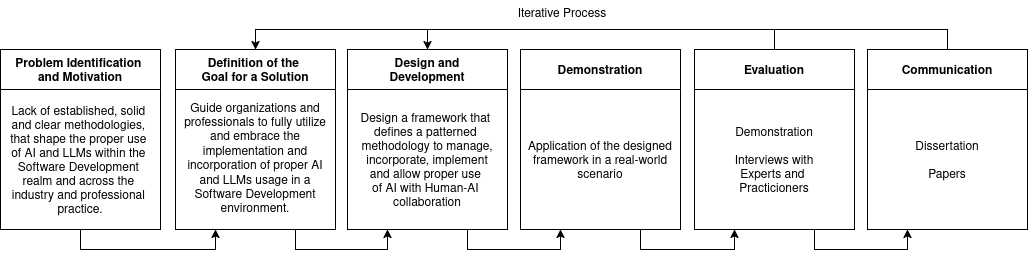
\includegraphics[width=1\linewidth]{./Images/dsrm.png}
    \caption{Phases of the Design Science Research Methodology}
    \label{fig:dsrm}
\end{figure}

\begin{itemize}
    \item \textbf{Problem Identification and Motivation:} This research addresses the lack of structured guidance, standardized methodologies, and evaluation practices for integrating AI and LLMs into software development while ensuring quality, accountability, and human oversight. This problem was identified through a Systematic Literature Review, which revealed fragmented practices and unclear human–AI role definitions across the SDLC. The motivation of this step is to map all AI related information to identify gaps informing both researchers and practitioners.
    \item \textbf{Definition of Objectives:} Based on the identified problem and the SLR findings, the research objectives aim to guide organizations in the effective, secure, and responsible adoption of AI and to maximize its potential use into an organized software environment through the definition of appropriate processes and governance mechanisms.
    \item \textbf{Design and Development:} Using the SLR findings as input, this step results in the design and construction of a process-oriented framework that defines phases, practices, roles, and decision points for human–AI collaboration across the SDLC.
    \item \textbf{Demonstration:} 
    This step will consist of applying the proposed framework in a realistic organizational scenario with a consultancy operating with Scrum practices and AI-augmented development techniques. The framework will be instantiated across a limited number of short development iterations, illustrating how it guides AI tool usage, prompt formulation, human–AI collaboration, validation checkpoints, and responsibility allocation throughout the SDLC. The main outputs of this step are documented development artifacts, decision rationales, and observations that show how the framework addresses the identified problem in practice.
    \item \textbf{Evaluation:} 
    The framework is applied in a realistic organizational scenario using Scrum-based and AI-augmented development practices, illustrating how it guides AI usage, collaboration, and validation throughout development iterations. Evidence from the demonstration and interviews will be synthesized to identify strengths, limitations, and opportunities for refinement, directly relating evaluation outcomes to the research objectives.
    \item \textbf{Communication:} This step will focus on disseminating the research results to both academic and professional audiences. This includes the preparation of the scientific article addressing the Systematic Literature Review, which will be submitted to the ACM Transactions on Software Engineering and Methodology journal; the submission of this report regarding the proposed framework along with the problem and its goals; and lastly the future development and submission of the final dissertation regarding the development of the framework.

\end{itemize}

% #############################################################################
\section{Mapping the Methodology onto this Document}
\label{sec:dsrm_mapping}

Because \ac{DSRM} prescribes activities rather than document sections, \Cref{tab:dsrm_chapter_mapping} states explicitly where each activity is carried out in this dissertation. The mapping is not strictly linear: as \Cref{chap:apex} describes, feedback gathered during the construction of the reference implementation fed back into the design of the framework, which is the iteration path \ac{DSRM} explicitly allows.

\begin{table}[H]
\centering
\caption{Mapping between DSRM activities and the chapters of this dissertation}
\label{tab:dsrm_chapter_mapping}
\begin{tabular}{p{4.6cm} p{3.2cm} p{6.4cm}}
\toprule
\textbf{DSRM Activity} & \textbf{Chapter} & \textbf{Output} \\
\midrule
Problem Identification and Motivation & \Cref{chap:slr,chap:problem} & Evidence base from the \ac{SLR}; formalised research problem \\
\addlinespace
Definition of Objectives & \Cref{chap:problem} & Objectives derived from the review findings \\
\addlinespace
Design and Development & \Cref{chap:proposal,chap:apex} & The framework, and Apex as its reference implementation \\
\addlinespace
Demonstration & \Cref{chap:demonstration} & Application of the artefact in a real-world project \\
\addlinespace
Evaluation & \Cref{chap:evaluation} & Usability and workload measurement, interviews, analytical assessment \\
\addlinespace
Communication & \Cref{chap:conclusion} & Publications and dissertation defence \\
\bottomrule
\end{tabular}
\end{table}
